\section{Results}
\label{sec:results}

\subsection{The agent versus existing methods}

\begin{table}[h]
\centering
\caption{Share of incidents where each method names the right component.}
\label{tab:baselines}
\begin{tabular}{lcc}
\toprule
Method & Right component & Also right fault type \\
\midrule
Statistical rule-based method & ${\sim}48\%$ & 38\% \\
Published academic method (BARO) & 46\% & not applicable \\
Trace-only academic methods & 0--5\% & not applicable \\
\textbf{Our LLM agent} & \textbf{83--87\%} & \textbf{48--57\%} \\
\bottomrule
\end{tabular}
\end{table}

The agent roughly doubles both usable baselines on finding the right component
(Table~\ref{tab:baselines}), at about one cent per diagnosis. Two supporting
observations make the case that an \emph{agent} specifically is needed: the two
non-LLM methods fail on \emph{different} fault types (so neither approach subsumes
the other), and simply feeding kernel data as extra columns into the academic method
changes nothing --- the value of the deep data is only accessible to something that
can reason about it.

\subsection{Thinning any one data source: no cliff}

\begin{table}[h]
\centering
\caption{Effect of thinning each data source (23 incidents per setting; ``fully
correct'' = right component and right fault type; measurement noise $\pm 9$ points).}
\label{tab:degradation}
\begin{tabular}{lll}
\toprule
Data source thinned & Range tested & Effect on accuracy \\
\midrule
Traces & keep 100\% down to 5\% & none (flat) \\
Metrics & every 5\,s down to every 60\,s & none (flat) \\
Logs & all lines down to errors only & none (flat) \\
Kernel & full detail down to absent & $-4$ points, but $+34\%$ more steps \\
\bottomrule
\end{tabular}
\end{table}

We expected accuracy to fall off a cliff somewhere. It does not
(Table~\ref{tab:degradation}, Fig.~\ref{fig:degradation}): across every thinning we
tested, accuracy stays inside the measurement-noise band, and 18 of 23 incidents give
the \emph{identical} outcome at every trace-thinning level. The reason is structural:
the agent's tools consume each data source as \emph{summaries} (latency percentiles,
rate changes, per-second aggregates), and summaries survive sampling; on top of that,
most faults leave fingerprints in more than one source, so when one channel thins,
the same signature is still visible in another.

\begin{figure}[h]
\centering
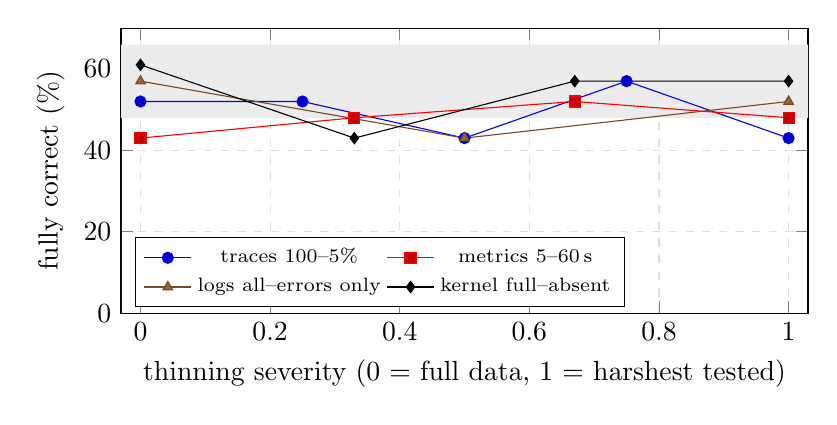
\begin{tikzpicture}
\begin{axis}[width=0.85\textwidth, height=5.2cm,
  xlabel={thinning severity (0 = full data, 1 = harshest tested)},
  ylabel={fully correct (\%)}, ymin=0, ymax=70, ytick={0,20,40,60},
  xmin=-0.03, xmax=1.03, legend style={font=\scriptsize, at={(0.02,0.02)},
  anchor=south west, legend columns=2}, grid=major, grid style={dashed,gray!25}]
\addplot[draw=none, fill=gray!15, forget plot] coordinates
  {(-0.03,48) (1.03,48) (1.03,66) (-0.03,66)} \closedcycle;
\addplot+[mark=*] coordinates {(0,52) (0.25,52) (0.5,43) (0.75,57) (1,43)};
\addlegendentry{traces 100--5\%}
\addplot+[mark=square*] coordinates {(0,43) (0.33,48) (0.67,52) (1,48)};
\addlegendentry{metrics 5--60\,s}
\addplot+[mark=triangle*] coordinates {(0,57) (0.5,43) (1,52)};
\addlegendentry{logs all--errors only}
\addplot+[mark=diamond*] coordinates {(0,61) (0.33,43) (0.67,57) (1,57)};
\addlegendentry{kernel full--absent}
\end{axis}
\end{tikzpicture}
\caption{Accuracy under per-source thinning. The shaded band is the measurement
noise around the full-data reference; no line leaves it in a consistent direction.
The one dip below the band is the ``kernel numbers without interpretation'' setting
discussed next.}
\label{fig:degradation}
\end{figure}

\subsection{What the kernel layer is actually worth}

\begin{table}[h]
\centering
\caption{Giving the agent different amounts of kernel data (23 incidents each).}
\label{tab:kernel}
\begin{tabular}{lccc}
\toprule
Kernel data provided & Right component & Fully correct & Steps per diagnosis \\
\midrule
Everything (numbers, waits, digests) & 83\% & 61\% & \textbf{9.1} \\
Raw numbers only & 74\% & \textbf{43\%} & 10.1 \\
English digests only & 78\% & 57\% & 10.0 \\
No kernel data at all & 78\% & 57\% & 12.2 \\
\bottomrule
\end{tabular}
\end{table}

Three findings (Table~\ref{tab:kernel}):
\begin{itemize}
  \item \textbf{Speed, not rescue.} Removing kernel data entirely costs almost no
  accuracy --- our improved tools over ordinary telemetry cover most faults --- but
  investigations take a third more steps. The kernel's dependable value is
  \emph{efficiency}.
  \item \textbf{One fault type genuinely needs it.} The slowed-database fault keeps
  its \emph{localization} without kernel data but loses its \emph{explanation}: only
  the kernel's wait analysis can say ``this database is idle yet all its time is
  spent waiting on something external --- the latency is imposed, not a bug''.
  \item \textbf{A partial view is worse than none.} Handing the model raw per-second
  kernel numbers without the interpretive layers produced the \emph{worst} result of
  the whole program --- worse than no kernel data at all. Uninterpreted deep data
  sends the model chasing noise. How you \emph{represent} a data source matters more
  than whether you have it.
\end{itemize}

\subsection{When a whole data source disappears}

Thinning is gentle; removal is not. Taking away \emph{traces entirely} (so the agent
cannot see who calls whom at all) is the first change that clearly hurts: accuracy
drops 14 points and effort rises 74\%, with the damage concentrated on faults whose
evidence is the shape of the call graph --- mostly in the larger, shared-database
application. Two silver linings: first, the slowed-database fault \emph{survives
trace removal} in the smaller application, because the kernel's wait analysis alone
carries it --- the clearest demonstration that the kernel layer acts as a backup
channel when ordinary telemetry is lost. Second, we checked whether kernel data
becomes more valuable as traces get \emph{thinner} (rather than absent): it does not
--- the backup role only activates on outright loss, which is consistent with
summaries surviving sampling.

\subsection{The minimum observability budget}

\begin{table}[h]
\centering
\caption{Combining all the cheap settings at once (23 incidents each).}
\label{tab:budget}
\begin{tabular}{lcccc}
\toprule
Monitoring setup & Right component & Fully correct & Steps & Data read per incident \\
\midrule
Everything (reference) & 83--87\% & 48--57\% & 9.0 & ${\sim}1.4$\,GB \\
Lean: 5\% traces, 60\,s metrics, errors-only logs & 78\% & 43\% & 7.6 & 24\,MB (\textbf{57$\times$ less}) \\
Minimal: lean, and no kernel & 83\% & 39\% & 11.0 & 12\,MB (115$\times$ less) \\
\bottomrule
\end{tabular}
\end{table}

Each cheap setting was individually free; combined (Table~\ref{tab:budget}) they are
\emph{almost} free: the lean setup reads 57$\times$ less data yet keeps over 90\% of
the agent's ability to name the right component. What suffers on a tight budget is
naming the exact fault \emph{type} --- the diagnosis gets vaguer before it gets
wrong. For teams deciding what to collect, the practical reading is: aggressive
sampling of traces, metrics and logs is safe for agent-assisted RCA; keep the kernel
layer if you care about explanations and investigation speed (it costs only half a
percent of throughput to record).

\subsection{The reusable-experience (skills) experiment}

\begin{table}[h]
\centering
\caption{Effect of the investigation-guide library (23 incidents each).}
\label{tab:skills}
\begin{tabular}{lcc}
\toprule
Setup & Right component & Fully correct \\
\midrule
No guides (agent from first principles) & 83\% & 57\% \\
With the evidence briefing (our standard setup) & \textbf{87\%} & \textbf{57\%} \\
Full guide library available & 78\% & 43\% \\
Library missing the matching guide (unseen fault) & 70\% & 39\% \\
\bottomrule
\end{tabular}
\end{table}

The idea: ship a library of short, human-written investigation guides, one per known
problem type, chosen automatically from the evidence. The result is instructive
(Table~\ref{tab:skills}): individual guides genuinely help --- one fault type is
solved \emph{only} when its guide is active, and the guides fixed several
fault-type confusions --- but the automatic \emph{selection} picks the right guide
only about two times in three, and a wrongly-chosen guide misleads more than no
guide. When the matching guide is missing entirely (our stand-in for a
never-seen-before problem), the selector almost never abstains as designed, and the
mismatched guides cost about 18 points versus just working from first principles.
The lesson is sharp: \emph{experience libraries are only as good as their selection
mechanism}, and that is the component to redesign --- the guides themselves, and the
agent's ability to override a bad one, both already work.

\subsection{How the agent's behaviour changes under degradation}

Because every step of every diagnosis is recorded, we can also watch \emph{how} the
agent works, not just whether it succeeds. Three observations: (1)~under thinning,
its behaviour barely changes --- nothing it relies on was lost; (2)~when a source is
removed, it compensates broadly, using \emph{all} remaining tools more rather than
switching to one substitute; and (3)~\textbf{effort rises before accuracy falls} ---
kernel removal costs $+34\%$ steps at almost no accuracy loss, trace removal $+74\%$
steps before the larger drop. In a real deployment, a rise in investigation effort
is therefore an early-warning signal that the monitoring setup has become
inadequate --- visible without knowing any ground truth. One operational quirk:
unless a tool states plainly ``this data source is unavailable'', the agent keeps
re-querying it service by service, wasting roughly a third of its steps; a one-line
tool change fixes this.

\subsection{A note on scoring fairness}

Some ``wrong fault type'' verdicts are arguably right: for a burst of injected
connection errors, the agent accurately describes connections being killed toward
the database but labels it an outage rather than an error storm --- a boundary in
our menu, not a misunderstanding. Scored with a conservative allowance for four such
documented boundary cases (and only when the component is also right), the
fully-correct rate rises from 52\% to 65\%. We report the strict number everywhere
and release all evidence text so a reader can judge.
